%!TEX root = main.tex
\chapter{User manual}
\label{cha:users_manual}

\section{Building the application}

To build the game you need a text editor of your choice (popular text editors include Eclipse IDE and IntelliJ IDEA) and the Android SDK version 8. These tools are available for Apple OSX, Microsoft Windows and Linux.
Alternatively, you could install and run the included \texttt{.apk} file. Doing this requires having a device running a compatible Android OS version.


\section{The rules}

\emph{Large and Heavily Armoured Warships} is a remake of the classic game Battleship, where two players are competing head to head in destroying their opponent's fleet of warships. In this version, each player is equipped with eight warships of differing sizes. Table \ref{tab:ship_distribution} shows our implementation's distribution of the different ships.

\vspace{0.5em}
\begin{table}
	\centering
	\label{tab:ship_distribution}
	\begin{tabular}{|l|l|l|}
		\hline
		\rowcolor[gray]{0.8}
		\bf{Type of ship} 	& \bf{Size} & \bf{Number of ships} \\
		\hline
		
		Aircraft carrier	& 5		& 1 \\
		Battleship 			& 4		& 2 \\
		Submarine			& 3		& 1 \\
		Destroyer			& 3		& 1 \\
		Patrol boat			& 2		& 3 \\
		\hline
	\end{tabular}

	\caption{Distribution of warships.}
\end{table}


\section{Playing the game}
The player starts the game by executing the application, and is then presented with the main menu screen (see figure \ref{fig:mainmenu} ) :
\begin{figure}[ht]
	\begin{minipage}[b]{0.325\linewidth}
		\centering
		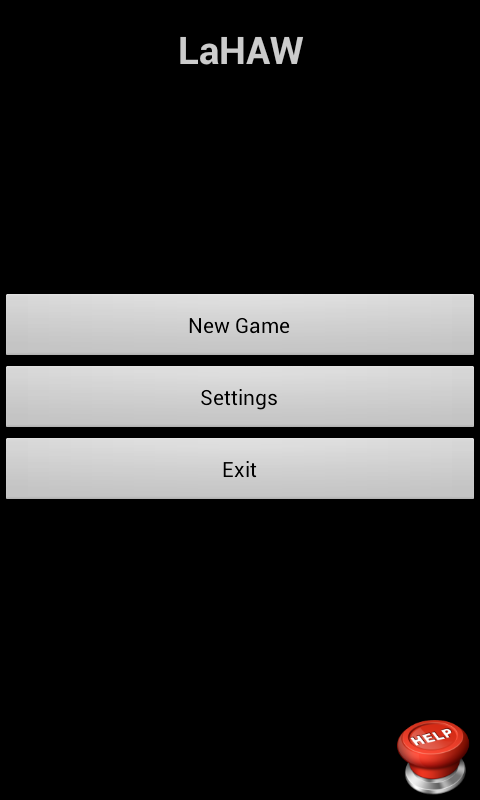
\includegraphics[scale=0.225]{img/Screenshot_MainMenu.png}
		\caption{Main menu      }
		\label{fig:mainmenu}
	\end{minipage}
	\begin{minipage}[b]{0.325\linewidth}
		\centering
		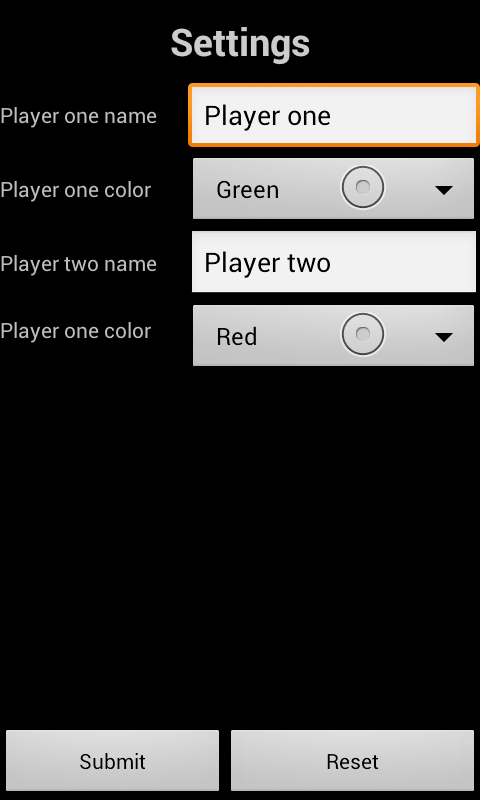
\includegraphics[scale=0.225]{img/Screenshot_settings.png}
		\caption{Settings}
		\label{fig:settings}
	\end{minipage}
	\begin{minipage}[b]{0.325\linewidth}
		\centering
		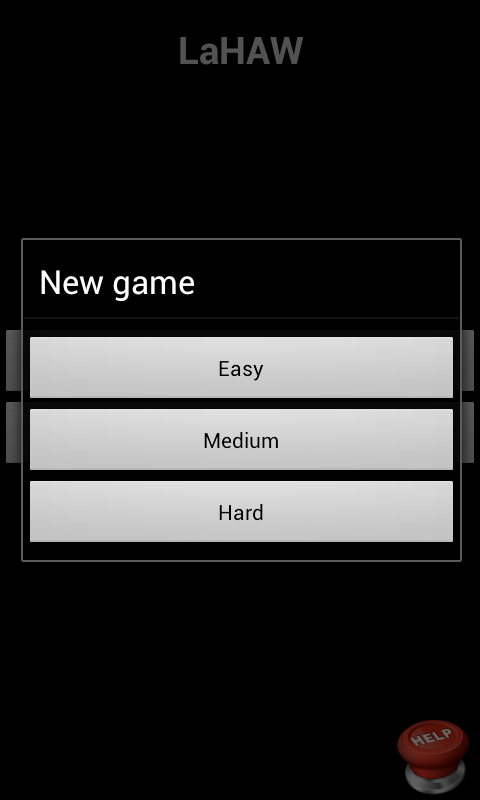
\includegraphics[scale=0.225]{img/Screenshot_difficulty.png}
		\caption{Difficulty}
		\label{fig:difficulty}
	\end{minipage}

\end{figure}

The main menu is quite straight-forward: From the main menu screen, the player faces three options: 
\noindent
\begin{itemize}
\item Start a new game
\item Edit game settings
\item Exit
\end{itemize}


In addition there is a help button in the lower right corner, should the user wish to ask the system for help\footnote{Note that the hint system is as of this prototype version implemented, but does not contain any actual hints at this time.}. 
Next the players would want to set their respective names and colours. Clicking the settings button will show the settings screen (see figure\ref{fig:settings}). At the settings screen, players can register and change their name, and also choose their preferred boat colour\footnote{Note that the boat colour is not used for anything in this prototype, but is stored on the device for future development of the application.}. 
Clicking the exit button will simply terminate the application. 

Clicking on the "New Game" button takes the player to the difficulty screen (see figure \ref{fig:difficulty}) . When arriving at this screen, the player can choose either "Easy" , "Medium" or "Hard" difficulty. Inexperienced players are advised to start with "Easy", and then move up as the they feel more confident and wants bigger challenge. 
In this version of the game, the difficulty dictates the size of the opponent's game board, with the easiest game mode having the least amount of bombable tiles than the harder modes. This setting is asymmetrical between the players\footnote{The setting is not asymmetrical in the prototype. Please see section \ref{sec:asym} for more information on this.}.
\newpage
When both players have chosen their name, colours and difficulty the game can begin. 
The warships are placed on preliminary starting positions when the game is started. The players can then change the placement of their respective boats by dragging the ships across the screen to their new location. If a player wishes to rotate one or more warships, this is done by holding down on a ship, and then touching the screen with another finger\footnote{We realise that this is a far from perfect way to accomplish the action, but it has been left in due to time constraints.}. After the player is happy with the placements, the game is started by pressing the "Start game" button in the upper left corner of the screen.

\begin{figure}[ht]
	\begin{minipage}[b]{0.325\linewidth}
		\centering
		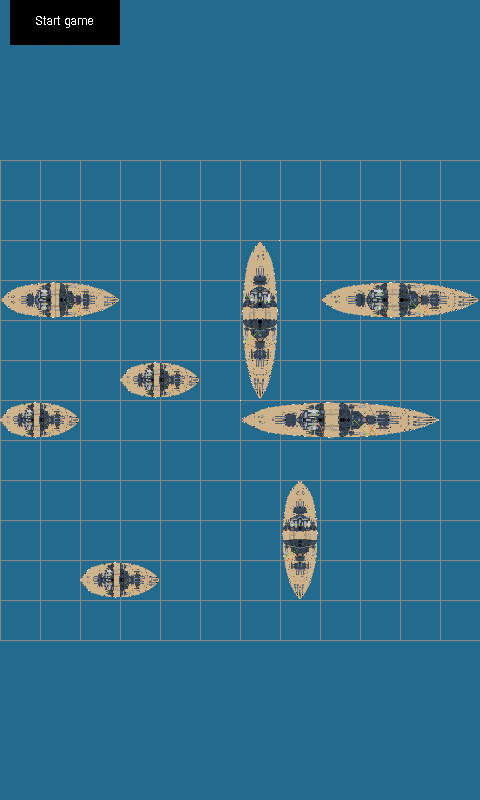
\includegraphics[scale=0.225]{img/Screenshot_placed.png}
		\caption{Boat placed}
		\label{fig:placed}
	\end{minipage}
	\begin{minipage}[b]{0.325\linewidth}
		\centering
		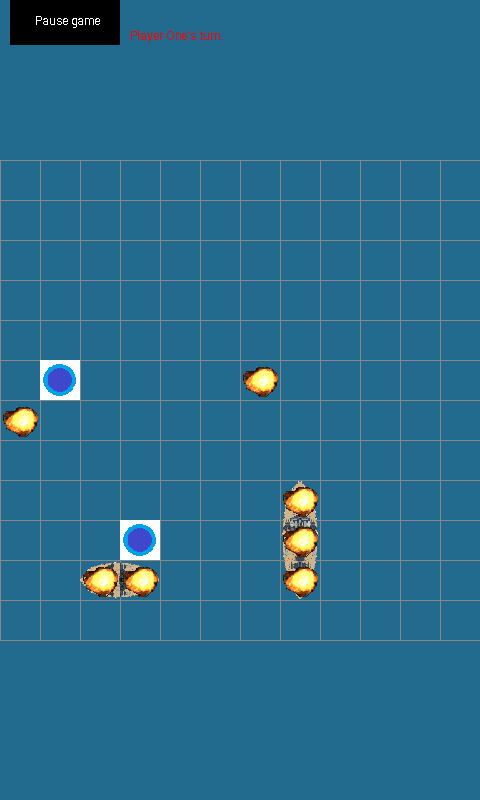
\includegraphics[scale=0.225]{img/Screenshot_bomb.png}
		\caption{Boat bombed}
		\label{fig:bomb}
	\end{minipage}
	\begin{minipage}[b]{0.325\linewidth}
		\centering
		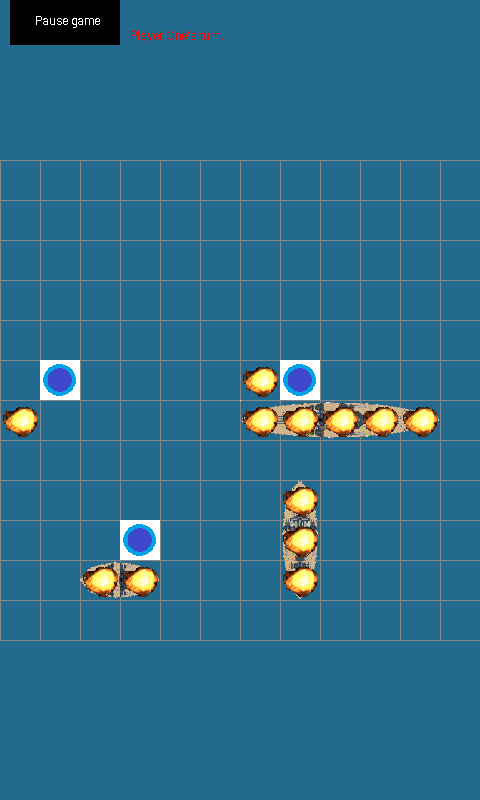
\includegraphics[scale=0.225]{img/Screenshot_sunk.png}
		\caption{Boat sunk}
		\label{fig:sunk}
	\end{minipage}

\end{figure}
When both players have placed and oriented their boats the next stage of the game can begin.
The game is turn-based, which means that the players takes turns to do their actions.
The game itself works so that each of the players take turns turn to guess the location of their opponent's warships. By tapping the screen on the desired location, a guess is made. If the opponent has a warship that occupies this location, a hit is registered and displayed on the screen (see figure \ref{fig:bomb}). When a player has guessed correctly and the whole warship is completely bombed, the entire warship is revealed (see figure \ref{fig:sunk}). After a guess has been made and the opponent gets its turn to guess a position. After a player's entire fleet has been demolished, the player with remaining warships is declared the winner. The user then accepts this outcome, and the game goes back to the main menu.

If the player wants to prematurely end or pause a game, the game can be paused by pressing the "Pause game" button at the upper left corner of the screen. This will present the player with two choices:
\noindent
\begin{itemize}
\item Resume the current game
\item Exit current game
\end{itemize} 
Exiting the game will bring the player to the game's main menu screen. 